\documentclass[twoside]{book}

% Packages required by doxygen
\usepackage{calc}
\usepackage{doxygen}
\usepackage{graphicx}
\usepackage[utf8]{inputenc}
\usepackage{makeidx}
\usepackage{multicol}
\usepackage{multirow}
\usepackage{textcomp}
\usepackage[table]{xcolor}

% Font selection
\usepackage[T1]{fontenc}
\usepackage{mathptmx}
\usepackage[scaled=.90]{helvet}
\usepackage{courier}
\usepackage{amssymb}
\usepackage{sectsty}
\renewcommand{\familydefault}{\sfdefault}
\allsectionsfont{%
  \fontseries{bc}\selectfont%
  \color{darkgray}%
}
\renewcommand{\DoxyLabelFont}{%
  \fontseries{bc}\selectfont%
  \color{darkgray}%
}

% Page & text layout
\usepackage{geometry}
\geometry{%
  a4paper,%
  top=2.5cm,%
  bottom=2.5cm,%
  left=2.5cm,%
  right=2.5cm%
}
\tolerance=750
\hfuzz=15pt
\hbadness=750
\setlength{\emergencystretch}{15pt}
\setlength{\parindent}{0cm}
\setlength{\parskip}{0.2cm}
\makeatletter
\renewcommand{\paragraph}{%
  \@startsection{paragraph}{4}{0ex}{-1.0ex}{1.0ex}{%
    \normalfont\normalsize\bfseries\SS@parafont%
  }%
}
\renewcommand{\subparagraph}{%
  \@startsection{subparagraph}{5}{0ex}{-1.0ex}{1.0ex}{%
    \normalfont\normalsize\bfseries\SS@subparafont%
  }%
}
\makeatother

% Headers & footers
\usepackage{fancyhdr}
\pagestyle{fancyplain}
\fancyhead[LE]{\fancyplain{}{\bfseries\thepage}}
\fancyhead[CE]{\fancyplain{}{}}
\fancyhead[RE]{\fancyplain{}{\bfseries\leftmark}}
\fancyhead[LO]{\fancyplain{}{\bfseries\rightmark}}
\fancyhead[CO]{\fancyplain{}{}}
\fancyhead[RO]{\fancyplain{}{\bfseries\thepage}}
\fancyfoot[LE]{\fancyplain{}{}}
\fancyfoot[CE]{\fancyplain{}{}}
\fancyfoot[RE]{\fancyplain{}{\bfseries\scriptsize Generated on Mon Nov 18 2013 01\-:47\-:46 for Lab 11 Heap -\/ Ernest Landrito by Doxygen }}
\fancyfoot[LO]{\fancyplain{}{\bfseries\scriptsize Generated on Mon Nov 18 2013 01\-:47\-:46 for Lab 11 Heap -\/ Ernest Landrito by Doxygen }}
\fancyfoot[CO]{\fancyplain{}{}}
\fancyfoot[RO]{\fancyplain{}{}}
\renewcommand{\footrulewidth}{0.4pt}
\renewcommand{\chaptermark}[1]{%
  \markboth{#1}{}%
}
\renewcommand{\sectionmark}[1]{%
  \markright{\thesection\ #1}%
}

% Indices & bibliography
\usepackage{natbib}
\usepackage[titles]{tocloft}
\setcounter{tocdepth}{3}
\setcounter{secnumdepth}{5}
\makeindex

% Hyperlinks (required, but should be loaded last)
\usepackage{ifpdf}
\ifpdf
  \usepackage[pdftex,pagebackref=true]{hyperref}
\else
  \usepackage[ps2pdf,pagebackref=true]{hyperref}
\fi
\hypersetup{%
  colorlinks=true,%
  linkcolor=blue,%
  citecolor=blue,%
  unicode%
}

% Custom commands
\newcommand{\clearemptydoublepage}{%
  \newpage{\pagestyle{empty}\cleardoublepage}%
}


%===== C O N T E N T S =====

\begin{document}

% Titlepage & ToC
\hypersetup{pageanchor=false}
\pagenumbering{roman}
\begin{titlepage}
\vspace*{7cm}
\begin{center}%
{\Large Lab 11 Heap -\/ Ernest Landrito }\\
\vspace*{1cm}
{\large Generated by Doxygen 1.8.5}\\
\vspace*{0.5cm}
{\small Mon Nov 18 2013 01:47:46}\\
\end{center}
\end{titlepage}
\clearemptydoublepage
\tableofcontents
\clearemptydoublepage
\pagenumbering{arabic}
\hypersetup{pageanchor=true}

%--- Begin generated contents ---
\chapter{Hierarchical Index}
\section{Class Hierarchy}
This inheritance list is sorted roughly, but not completely, alphabetically\-:\begin{DoxyCompactList}
\item \contentsline{section}{Greater$<$ Key\-Type $>$}{\pageref{class_greater}}{}
\item \contentsline{section}{Heap$<$ Data\-Type, Key\-Type, Comparator $>$}{\pageref{class_heap}}{}
\item \contentsline{section}{Heap$<$ Data\-Type $>$}{\pageref{class_heap}}{}
\begin{DoxyCompactList}
\item \contentsline{section}{Priority\-Queue$<$ Data\-Type, Key\-Type, Comparator $>$}{\pageref{class_priority_queue}}{}
\end{DoxyCompactList}
\item \contentsline{section}{Less$<$ Key\-Type $>$}{\pageref{class_less}}{}
\item \contentsline{section}{Less$<$ int $>$}{\pageref{class_less}}{}
\item \contentsline{section}{Task\-Data}{\pageref{struct_task_data}}{}
\item \contentsline{section}{Test\-Data}{\pageref{class_test_data}}{}
\item \contentsline{section}{Test\-Data\-Item$<$ Key\-Type $>$}{\pageref{class_test_data_item}}{}
\end{DoxyCompactList}

\chapter{Class Index}
\section{Class List}
Here are the classes, structs, unions and interfaces with brief descriptions\-:\begin{DoxyCompactList}
\item\contentsline{section}{\hyperlink{classbinary_search}{binary\-Search} }{\pageref{classbinary_search}}{}
\item\contentsline{section}{\hyperlink{classlinear_search}{linear\-Search} }{\pageref{classlinear_search}}{}
\item\contentsline{section}{\hyperlink{class_search}{Search} }{\pageref{class_search}}{}
\item\contentsline{section}{\hyperlink{class_s_t_l_search}{S\-T\-L\-Search} }{\pageref{class_s_t_l_search}}{}
\item\contentsline{section}{\hyperlink{class_test_vector}{Test\-Vector} }{\pageref{class_test_vector}}{}
\item\contentsline{section}{\hyperlink{class_timer}{Timer} }{\pageref{class_timer}}{}
\end{DoxyCompactList}

\chapter{File Index}
\section{File List}
Here is a list of all files with brief descriptions\-:\begin{DoxyCompactList}
\item\contentsline{section}{\hyperlink{config_8h}{config.\-h} }{\pageref{config_8h}}{}
\item\contentsline{section}{\hyperlink{constructor_8cpp}{constructor.\-cpp} }{\pageref{constructor_8cpp}}{}
\item\contentsline{section}{\hyperlink{inc_8cpp}{inc.\-cpp} }{\pageref{inc_8cpp}}{}
\item\contentsline{section}{\hyperlink{search_8cpp}{search.\-cpp} }{\pageref{search_8cpp}}{}
\item\contentsline{section}{\hyperlink{sort_8cpp}{sort.\-cpp} }{\pageref{sort_8cpp}}{}
\item\contentsline{section}{\hyperlink{test_8cpp}{test.\-cpp} }{\pageref{test_8cpp}}{}
\item\contentsline{section}{\hyperlink{test13_8cpp}{test13.\-cpp} }{\pageref{test13_8cpp}}{}
\item\contentsline{section}{\hyperlink{testtimer_8c_09_09}{testtimer.\-c++} }{\pageref{testtimer_8c_09_09}}{}
\item\contentsline{section}{\hyperlink{testtimer_8cc}{testtimer.\-cc} }{\pageref{testtimer_8cc}}{}
\item\contentsline{section}{\hyperlink{testtimer_8cpp}{testtimer.\-cpp} }{\pageref{testtimer_8cpp}}{}
\item\contentsline{section}{\hyperlink{testvector_8cpp}{testvector.\-cpp} }{\pageref{testvector_8cpp}}{}
\item\contentsline{section}{\hyperlink{testvector_8h}{testvector.\-h} }{\pageref{testvector_8h}}{}
\item\contentsline{section}{\hyperlink{text_8cc}{text.\-cc} }{\pageref{text_8cc}}{}
\item\contentsline{section}{\hyperlink{_timer_8cpp}{Timer.\-cpp} }{\pageref{_timer_8cpp}}{}
\item\contentsline{section}{\hyperlink{_timer_8cs}{Timer.\-cs} }{\pageref{_timer_8cs}}{}
\item\contentsline{section}{\hyperlink{_timer_8h}{Timer.\-h} }{\pageref{_timer_8h}}{}
\end{DoxyCompactList}

\chapter{Class Documentation}
\hypertarget{class_greater}{\section{Greater$<$ Key\-Type $>$ Class Template Reference}
\label{class_greater}\index{Greater$<$ Key\-Type $>$@{Greater$<$ Key\-Type $>$}}
}
\subsection*{Public Member Functions}
\begin{DoxyCompactItemize}
\item 
bool \hyperlink{class_greater_a79d9cb7121723ee9d65b11cb2fce0379}{operator()} (const Key\-Type \&a, const Key\-Type \&b) const 
\end{DoxyCompactItemize}


\subsection{Member Function Documentation}
\hypertarget{class_greater_a79d9cb7121723ee9d65b11cb2fce0379}{\index{Greater@{Greater}!operator()@{operator()}}
\index{operator()@{operator()}!Greater@{Greater}}
\subsubsection[{operator()}]{\setlength{\rightskip}{0pt plus 5cm}template$<$typename Key\-Type  = int$>$ bool {\bf Greater}$<$ Key\-Type $>$\-::operator() (
\begin{DoxyParamCaption}
\item[{const Key\-Type \&}]{a, }
\item[{const Key\-Type \&}]{b}
\end{DoxyParamCaption}
) const\hspace{0.3cm}{\ttfamily [inline]}}}\label{class_greater_a79d9cb7121723ee9d65b11cb2fce0379}


The documentation for this class was generated from the following file\-:\begin{DoxyCompactItemize}
\item 
\hyperlink{test11_8cpp}{test11.\-cpp}\end{DoxyCompactItemize}

\hypertarget{class_heap}{\section{Heap$<$ Data\-Type, Key\-Type, Comparator $>$ Class Template Reference}
\label{class_heap}\index{Heap$<$ Data\-Type, Key\-Type, Comparator $>$@{Heap$<$ Data\-Type, Key\-Type, Comparator $>$}}
}


{\ttfamily \#include $<$Heap.\-h$>$}

\subsection*{Public Member Functions}
\begin{DoxyCompactItemize}
\item 
\hyperlink{class_heap_ae17e34e3c86d88263a8fdf80b9ba78fc}{Heap} (int max\-Number=\hyperlink{class_heap_a967c19732a20a72e8e824402ad6763c8}{D\-E\-F\-A\-U\-L\-T\-\_\-\-M\-A\-X\-\_\-\-H\-E\-A\-P\-\_\-\-S\-I\-Z\-E})
\item 
\hyperlink{class_heap_a97e3b462be1c6af31d7519546bba8907}{Heap} (const \hyperlink{class_heap}{Heap} \&other)
\item 
\hyperlink{class_heap}{Heap} \& \hyperlink{class_heap_a5ed119341c39bcea1437321d4247dd40}{operator=} (const \hyperlink{class_heap}{Heap} \&other)
\item 
\hyperlink{class_heap_a555ade7891007de959bef0ee53e28767}{$\sim$\-Heap} ()
\item 
void \hyperlink{class_heap_aa68cf80454ab1b246fa723612805a91e}{insert} (const Data\-Type \&new\-Data\-Item)  throw ( logic\-\_\-error )
\item 
Data\-Type \hyperlink{class_heap_a4a18bfdacd897c45fc3da13f22b8930d}{remove} ()  throw ( logic\-\_\-error )
\item 
void \hyperlink{class_heap_a19a78c8eae2cf7c8253e34e54d86ed73}{clear} ()
\item 
bool \hyperlink{class_heap_ab8fa26d416ac0e27dfcbf18c54f8f73f}{is\-Empty} () const 
\item 
bool \hyperlink{class_heap_ac9111b884c74a376240e0155a788756e}{is\-Full} () const 
\item 
void \hyperlink{class_heap_a3ae1e1f27a145749c8b9f2da777cb8bc}{show\-Structure} () const 
\item 
void \hyperlink{class_heap_a4bdb1772ea92899de245d6cbd217d085}{write\-Levels} () const 
\end{DoxyCompactItemize}
\subsection*{Static Public Attributes}
\begin{DoxyCompactItemize}
\item 
static const int \hyperlink{class_heap_a967c19732a20a72e8e824402ad6763c8}{D\-E\-F\-A\-U\-L\-T\-\_\-\-M\-A\-X\-\_\-\-H\-E\-A\-P\-\_\-\-S\-I\-Z\-E} = 10
\end{DoxyCompactItemize}


\subsection{Constructor \& Destructor Documentation}
\hypertarget{class_heap_ae17e34e3c86d88263a8fdf80b9ba78fc}{\index{Heap@{Heap}!Heap@{Heap}}
\index{Heap@{Heap}!Heap@{Heap}}
\subsubsection[{Heap}]{\setlength{\rightskip}{0pt plus 5cm}template$<$typename Data\-Type , typename Key\-Type , typename Comparator $>$ {\bf Heap}$<$ Data\-Type, Key\-Type, Comparator $>$\-::{\bf Heap} (
\begin{DoxyParamCaption}
\item[{int}]{max\-Number = {\ttfamily {\bf D\-E\-F\-A\-U\-L\-T\-\_\-\-M\-A\-X\-\_\-\-H\-E\-A\-P\-\_\-\-S\-I\-Z\-E}}}
\end{DoxyParamCaption}
)}}\label{class_heap_ae17e34e3c86d88263a8fdf80b9ba78fc}
\begin{DoxyPrecond}{Precondition}
New \hyperlink{class_heap}{Heap} Class 
\end{DoxyPrecond}
\begin{DoxyPostcond}{Postcondition}
dynamically allocated array of size max\-Number 
\end{DoxyPostcond}

\begin{DoxyParams}{Parameters}
{\em max\-Number} & the size of the array to be formed\\
\hline
\end{DoxyParams}
Algorithm\-:
\begin{DoxyItemize}
\item set size to zero
\item set max\-Size
\item allocate array
\end{DoxyItemize}

Exceptional/\-Error Conditions\-:
\begin{DoxyItemize}
\item none 
\end{DoxyItemize}\hypertarget{class_heap_a97e3b462be1c6af31d7519546bba8907}{\index{Heap@{Heap}!Heap@{Heap}}
\index{Heap@{Heap}!Heap@{Heap}}
\subsubsection[{Heap}]{\setlength{\rightskip}{0pt plus 5cm}template$<$typename Data\-Type , typename Key\-Type , typename Comparator $>$ {\bf Heap}$<$ Data\-Type, Key\-Type, Comparator $>$\-::{\bf Heap} (
\begin{DoxyParamCaption}
\item[{const {\bf Heap}$<$ Data\-Type, Key\-Type, Comparator $>$ \&}]{other}
\end{DoxyParamCaption}
)}}\label{class_heap_a97e3b462be1c6af31d7519546bba8907}
\begin{DoxyPrecond}{Precondition}
new \hyperlink{class_heap}{Heap} class
\end{DoxyPrecond}
\begin{DoxyPostcond}{Postcondition}
a deep copy of source \hyperlink{class_heap}{Heap}
\end{DoxyPostcond}

\begin{DoxyParams}{Parameters}
{\em other} & Source Hash\-Table to be deep copied\\
\hline
\end{DoxyParams}
Algorithm\-:
\begin{DoxyItemize}
\item Use overloaded assignment operator to copy the data from the source to this class 
\end{DoxyItemize}\hypertarget{class_heap_a555ade7891007de959bef0ee53e28767}{\index{Heap@{Heap}!$\sim$\-Heap@{$\sim$\-Heap}}
\index{$\sim$\-Heap@{$\sim$\-Heap}!Heap@{Heap}}
\subsubsection[{$\sim$\-Heap}]{\setlength{\rightskip}{0pt plus 5cm}template$<$typename Data\-Type , typename Key\-Type , typename Comparator $>$ {\bf Heap}$<$ Data\-Type, Key\-Type, Comparator $>$\-::$\sim${\bf Heap} (
\begin{DoxyParamCaption}
{}
\end{DoxyParamCaption}
)}}\label{class_heap_a555ade7891007de959bef0ee53e28767}
\begin{DoxyPrecond}{Precondition}
a \hyperlink{class_heap}{Heap}
\end{DoxyPrecond}
\begin{DoxyPostcond}{Postcondition}
deallocated \hyperlink{class_heap}{Heap}
\end{DoxyPostcond}
Algorithm\-:
\begin{DoxyItemize}
\item Use clear member function to deallocate the Hash\-Table
\item delete the array 
\end{DoxyItemize}

\subsection{Member Function Documentation}
\hypertarget{class_heap_a19a78c8eae2cf7c8253e34e54d86ed73}{\index{Heap@{Heap}!clear@{clear}}
\index{clear@{clear}!Heap@{Heap}}
\subsubsection[{clear}]{\setlength{\rightskip}{0pt plus 5cm}template$<$typename Data\-Type , typename Key\-Type , typename Comparator $>$ void {\bf Heap}$<$ Data\-Type, Key\-Type, Comparator $>$\-::clear (
\begin{DoxyParamCaption}
{}
\end{DoxyParamCaption}
)}}\label{class_heap_a19a78c8eae2cf7c8253e34e54d86ed73}
\begin{DoxyPrecond}{Precondition}
a \hyperlink{class_heap}{Heap}
\end{DoxyPrecond}
\begin{DoxyPostcond}{Postcondition}
an empty heap
\end{DoxyPostcond}
Algorithm\-:
\begin{DoxyItemize}
\item set the size of the heap to 0; 
\end{DoxyItemize}\hypertarget{class_heap_aa68cf80454ab1b246fa723612805a91e}{\index{Heap@{Heap}!insert@{insert}}
\index{insert@{insert}!Heap@{Heap}}
\subsubsection[{insert}]{\setlength{\rightskip}{0pt plus 5cm}template$<$typename Data\-Type, typename Key\-Type , typename Comparator $>$ void {\bf Heap}$<$ Data\-Type, Key\-Type, Comparator $>$\-::insert (
\begin{DoxyParamCaption}
\item[{const Data\-Type \&}]{new\-Data\-Item}
\end{DoxyParamCaption}
) throw  logic\-\_\-error) }}\label{class_heap_aa68cf80454ab1b246fa723612805a91e}
\begin{DoxyPrecond}{Precondition}
a \hyperlink{class_heap}{Heap}
\end{DoxyPrecond}
\begin{DoxyPostcond}{Postcondition}
a new node inserted into the B\-S\-Tree at the appropriate array location of the \hyperlink{class_heap}{Heap}
\end{DoxyPostcond}

\begin{DoxyParams}{Parameters}
{\em new\-Data\-Item} & Data to be inserted into the \hyperlink{class_heap}{Heap}\\
\hline
\end{DoxyParams}
Algorithm\-:
\begin{DoxyItemize}
\item if the array isn't full
\item loop until the compare is no longer fulfilled
\item move the node up the tree if compare is fulfilled
\item increase list size 
\end{DoxyItemize}\hypertarget{class_heap_ab8fa26d416ac0e27dfcbf18c54f8f73f}{\index{Heap@{Heap}!is\-Empty@{is\-Empty}}
\index{is\-Empty@{is\-Empty}!Heap@{Heap}}
\subsubsection[{is\-Empty}]{\setlength{\rightskip}{0pt plus 5cm}template$<$typename Data\-Type , typename Key\-Type , typename Comparator $>$ bool {\bf Heap}$<$ Data\-Type, Key\-Type, Comparator $>$\-::is\-Empty (
\begin{DoxyParamCaption}
{}
\end{DoxyParamCaption}
) const}}\label{class_heap_ab8fa26d416ac0e27dfcbf18c54f8f73f}
\begin{DoxyPrecond}{Precondition}
a \hyperlink{class_heap}{Heap}
\end{DoxyPrecond}
\begin{DoxyPostcond}{Postcondition}
returns if the heap is empty
\end{DoxyPostcond}
\begin{DoxyReturn}{Returns}
returns if the heap is empty
\end{DoxyReturn}
Algorithm\-:
\begin{DoxyItemize}
\item return if the size is equal to 0 
\end{DoxyItemize}\hypertarget{class_heap_ac9111b884c74a376240e0155a788756e}{\index{Heap@{Heap}!is\-Full@{is\-Full}}
\index{is\-Full@{is\-Full}!Heap@{Heap}}
\subsubsection[{is\-Full}]{\setlength{\rightskip}{0pt plus 5cm}template$<$typename Data\-Type , typename Key\-Type , typename Comparator $>$ bool {\bf Heap}$<$ Data\-Type, Key\-Type, Comparator $>$\-::is\-Full (
\begin{DoxyParamCaption}
{}
\end{DoxyParamCaption}
) const}}\label{class_heap_ac9111b884c74a376240e0155a788756e}
\begin{DoxyPrecond}{Precondition}
a \hyperlink{class_heap}{Heap}
\end{DoxyPrecond}
\begin{DoxyPostcond}{Postcondition}
returns if the heap is full
\end{DoxyPostcond}
\begin{DoxyReturn}{Returns}
returns if the heap is full
\end{DoxyReturn}
Algorithm\-:
\begin{DoxyItemize}
\item return if the size is equal to the max size 
\end{DoxyItemize}\hypertarget{class_heap_a5ed119341c39bcea1437321d4247dd40}{\index{Heap@{Heap}!operator=@{operator=}}
\index{operator=@{operator=}!Heap@{Heap}}
\subsubsection[{operator=}]{\setlength{\rightskip}{0pt plus 5cm}template$<$typename Data\-Type , typename Key\-Type , typename Comparator $>$ {\bf Heap}$<$ Data\-Type, Key\-Type, Comparator $>$ \& {\bf Heap}$<$ Data\-Type, Key\-Type, Comparator $>$\-::operator= (
\begin{DoxyParamCaption}
\item[{const {\bf Heap}$<$ Data\-Type, Key\-Type, Comparator $>$ \&}]{other}
\end{DoxyParamCaption}
)}}\label{class_heap_a5ed119341c39bcea1437321d4247dd40}
\begin{DoxyPrecond}{Precondition}
a \hyperlink{class_heap}{Heap} class
\end{DoxyPrecond}
\begin{DoxyPostcond}{Postcondition}
a deep copy of source heap
\end{DoxyPostcond}

\begin{DoxyParams}{Parameters}
{\em source} & Source \hyperlink{class_heap}{Heap} to be deep copied\\
\hline
\end{DoxyParams}
Algorithm\-:
\begin{DoxyItemize}
\item if the heap is not empt and it isnt itself clear the heap
\item copy the data 
\end{DoxyItemize}\hypertarget{class_heap_a4a18bfdacd897c45fc3da13f22b8930d}{\index{Heap@{Heap}!remove@{remove}}
\index{remove@{remove}!Heap@{Heap}}
\subsubsection[{remove}]{\setlength{\rightskip}{0pt plus 5cm}template$<$typename Data\-Type , typename Key\-Type , typename Comparator $>$ Data\-Type {\bf Heap}$<$ Data\-Type, Key\-Type, Comparator $>$\-::remove (
\begin{DoxyParamCaption}
{}
\end{DoxyParamCaption}
) throw  logic\-\_\-error) }}\label{class_heap_a4a18bfdacd897c45fc3da13f22b8930d}
\begin{DoxyPrecond}{Precondition}
a \hyperlink{class_heap}{Heap}
\end{DoxyPrecond}
\begin{DoxyPostcond}{Postcondition}
\hyperlink{class_heap}{Heap} with root node removed
\end{DoxyPostcond}
\begin{DoxyReturn}{Returns}
returns the data at the front of the array
\end{DoxyReturn}
Algorithm\-:
\begin{DoxyItemize}
\item Throw the logic error if the heap is empty
\item reduce size
\item set return value
\item move the item at the end of the list to the front
\item move the data item down through the list switching with things it compares to 
\end{DoxyItemize}\hypertarget{class_heap_a3ae1e1f27a145749c8b9f2da777cb8bc}{\index{Heap@{Heap}!show\-Structure@{show\-Structure}}
\index{show\-Structure@{show\-Structure}!Heap@{Heap}}
\subsubsection[{show\-Structure}]{\setlength{\rightskip}{0pt plus 5cm}template$<$typename Data\-Type , typename Key\-Type , typename Comparator $>$ void {\bf Heap}$<$ Data\-Type, Key\-Type, Comparator $>$\-::show\-Structure (
\begin{DoxyParamCaption}
{}
\end{DoxyParamCaption}
) const}}\label{class_heap_a3ae1e1f27a145749c8b9f2da777cb8bc}
\hypertarget{class_heap_a4bdb1772ea92899de245d6cbd217d085}{\index{Heap@{Heap}!write\-Levels@{write\-Levels}}
\index{write\-Levels@{write\-Levels}!Heap@{Heap}}
\subsubsection[{write\-Levels}]{\setlength{\rightskip}{0pt plus 5cm}template$<$typename Data\-Type , typename Key\-Type , typename Comparator $>$ void {\bf Heap}$<$ Data\-Type, Key\-Type, Comparator $>$\-::write\-Levels (
\begin{DoxyParamCaption}
{}
\end{DoxyParamCaption}
) const}}\label{class_heap_a4bdb1772ea92899de245d6cbd217d085}
\begin{DoxyPrecond}{Precondition}
a \hyperlink{class_heap}{Heap}
\end{DoxyPrecond}
\begin{DoxyPostcond}{Postcondition}
prints each level of the heap
\end{DoxyPostcond}
Algorithm\-:
\begin{DoxyItemize}
\item set how many to print per level to 1
\item set how many printed to 0
\item loop until the every item is printed;
\item after printing each level multiply to print by 2 and return printed counter to 0 
\end{DoxyItemize}

\subsection{Member Data Documentation}
\hypertarget{class_heap_a967c19732a20a72e8e824402ad6763c8}{\index{Heap@{Heap}!D\-E\-F\-A\-U\-L\-T\-\_\-\-M\-A\-X\-\_\-\-H\-E\-A\-P\-\_\-\-S\-I\-Z\-E@{D\-E\-F\-A\-U\-L\-T\-\_\-\-M\-A\-X\-\_\-\-H\-E\-A\-P\-\_\-\-S\-I\-Z\-E}}
\index{D\-E\-F\-A\-U\-L\-T\-\_\-\-M\-A\-X\-\_\-\-H\-E\-A\-P\-\_\-\-S\-I\-Z\-E@{D\-E\-F\-A\-U\-L\-T\-\_\-\-M\-A\-X\-\_\-\-H\-E\-A\-P\-\_\-\-S\-I\-Z\-E}!Heap@{Heap}}
\subsubsection[{D\-E\-F\-A\-U\-L\-T\-\_\-\-M\-A\-X\-\_\-\-H\-E\-A\-P\-\_\-\-S\-I\-Z\-E}]{\setlength{\rightskip}{0pt plus 5cm}template$<$typename Data\-Type, typename Key\-Type = int, typename Comparator = Less$<$\-Key\-Type$>$$>$ const int {\bf Heap}$<$ Data\-Type, Key\-Type, Comparator $>$\-::D\-E\-F\-A\-U\-L\-T\-\_\-\-M\-A\-X\-\_\-\-H\-E\-A\-P\-\_\-\-S\-I\-Z\-E = 10\hspace{0.3cm}{\ttfamily [static]}}}\label{class_heap_a967c19732a20a72e8e824402ad6763c8}


The documentation for this class was generated from the following files\-:\begin{DoxyCompactItemize}
\item 
\hyperlink{_heap_8h}{Heap.\-h}\item 
\hyperlink{_heap_8cpp}{Heap.\-cpp}\item 
\hyperlink{_heap2_8cpp}{Heap2.\-cpp}\item 
\hyperlink{show11_8cpp}{show11.\-cpp}\end{DoxyCompactItemize}

\hypertarget{class_less}{\section{Less$<$ Key\-Type $>$ Class Template Reference}
\label{class_less}\index{Less$<$ Key\-Type $>$@{Less$<$ Key\-Type $>$}}
}


{\ttfamily \#include $<$Heap.\-h$>$}

\subsection*{Public Member Functions}
\begin{DoxyCompactItemize}
\item 
bool \hyperlink{class_less_afee76a5248eb9c6c8fd1f005360d44d5}{operator()} (const Key\-Type \&a, const Key\-Type \&b) const 
\end{DoxyCompactItemize}


\subsection{Member Function Documentation}
\hypertarget{class_less_afee76a5248eb9c6c8fd1f005360d44d5}{\index{Less@{Less}!operator()@{operator()}}
\index{operator()@{operator()}!Less@{Less}}
\subsubsection[{operator()}]{\setlength{\rightskip}{0pt plus 5cm}template$<$typename Key\-Type = int$>$ bool {\bf Less}$<$ Key\-Type $>$\-::operator() (
\begin{DoxyParamCaption}
\item[{const Key\-Type \&}]{a, }
\item[{const Key\-Type \&}]{b}
\end{DoxyParamCaption}
) const\hspace{0.3cm}{\ttfamily [inline]}}}\label{class_less_afee76a5248eb9c6c8fd1f005360d44d5}


The documentation for this class was generated from the following file\-:\begin{DoxyCompactItemize}
\item 
\hyperlink{_heap_8h}{Heap.\-h}\end{DoxyCompactItemize}

\hypertarget{class_priority_queue}{\section{Priority\-Queue$<$ Data\-Type, Key\-Type, Comparator $>$ Class Template Reference}
\label{class_priority_queue}\index{Priority\-Queue$<$ Data\-Type, Key\-Type, Comparator $>$@{Priority\-Queue$<$ Data\-Type, Key\-Type, Comparator $>$}}
}


{\ttfamily \#include $<$Priority\-Queue.\-h$>$}

Inheritance diagram for Priority\-Queue$<$ Data\-Type, Key\-Type, Comparator $>$\-:\begin{figure}[H]
\begin{center}
\leavevmode
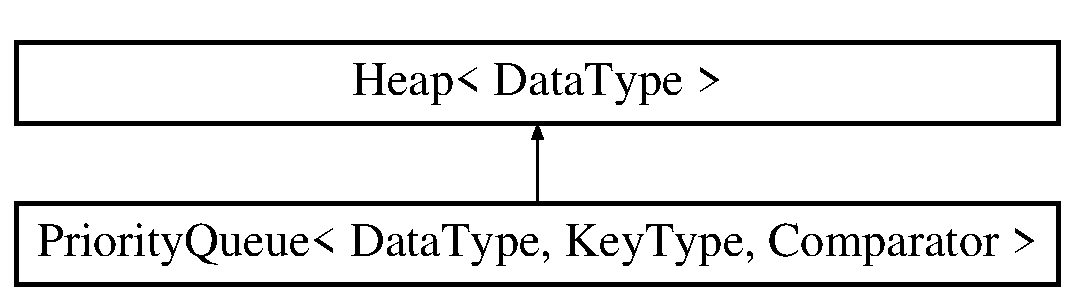
\includegraphics[height=2.000000cm]{class_priority_queue}
\end{center}
\end{figure}
\subsection*{Public Member Functions}
\begin{DoxyCompactItemize}
\item 
\hyperlink{class_priority_queue_a47de2a46cff1d6a6ed30a99c94dc1b14}{Priority\-Queue} (int max\-Number=\hyperlink{_priority_queue_8h_a88703212007be018800be64f2f5fde2f}{def\-Max\-Queue\-Size})
\item 
\hyperlink{class_priority_queue_ab3b8c46007394fe44868b316ec157b92}{Priority\-Queue} (const \hyperlink{class_heap}{Heap}$<$ Data\-Type, Key\-Type, Comparator $>$ \&other)
\item 
\hyperlink{class_priority_queue}{Priority\-Queue} \& \hyperlink{class_priority_queue_ad4a011c82e41027ff8c2b55fe1923b33}{operator=} (const \hyperlink{class_priority_queue}{Priority\-Queue} \&other)
\item 
\hyperlink{class_priority_queue_a7d959dc823b18c647aa0ee4a80f27881}{$\sim$\-Priority\-Queue} ()
\item 
void \hyperlink{class_priority_queue_a61f3339cf0e87c67ed004f8eff0a1bfa}{enqueue} (const Data\-Type \&new\-Data\-Item)
\item 
Data\-Type \hyperlink{class_priority_queue_a5bc758e313d6244e672ea6e81d695a46}{dequeue} ()
\item 
void \hyperlink{class_priority_queue_a8386c8ea2b5806646cc7de9dd1b8df4b}{clear} ()
\item 
bool \hyperlink{class_priority_queue_a8cc481ad399a3117de6b1779a9d3edfe}{is\-Empty} ()
\item 
bool \hyperlink{class_priority_queue_a959aa69891bcbf024674ceaf527eeeec}{is\-Full} ()
\end{DoxyCompactItemize}
\subsection*{Additional Inherited Members}


\subsection{Constructor \& Destructor Documentation}
\hypertarget{class_priority_queue_a47de2a46cff1d6a6ed30a99c94dc1b14}{\index{Priority\-Queue@{Priority\-Queue}!Priority\-Queue@{Priority\-Queue}}
\index{Priority\-Queue@{Priority\-Queue}!PriorityQueue@{Priority\-Queue}}
\subsubsection[{Priority\-Queue}]{\setlength{\rightskip}{0pt plus 5cm}template$<$typename Data\-Type , typename Key\-Type  = int, typename Comparator  = Less$<$\-Key\-Type$>$$>$ {\bf Priority\-Queue}$<$ Data\-Type, Key\-Type, Comparator $>$\-::{\bf Priority\-Queue} (
\begin{DoxyParamCaption}
\item[{int}]{max\-Number = {\ttfamily {\bf def\-Max\-Queue\-Size}}}
\end{DoxyParamCaption}
)\hspace{0.3cm}{\ttfamily [inline]}}}\label{class_priority_queue_a47de2a46cff1d6a6ed30a99c94dc1b14}
\hypertarget{class_priority_queue_ab3b8c46007394fe44868b316ec157b92}{\index{Priority\-Queue@{Priority\-Queue}!Priority\-Queue@{Priority\-Queue}}
\index{Priority\-Queue@{Priority\-Queue}!PriorityQueue@{Priority\-Queue}}
\subsubsection[{Priority\-Queue}]{\setlength{\rightskip}{0pt plus 5cm}template$<$typename Data\-Type , typename Key\-Type  = int, typename Comparator  = Less$<$\-Key\-Type$>$$>$ {\bf Priority\-Queue}$<$ Data\-Type, Key\-Type, Comparator $>$\-::{\bf Priority\-Queue} (
\begin{DoxyParamCaption}
\item[{const {\bf Heap}$<$ Data\-Type, Key\-Type, Comparator $>$ \&}]{other}
\end{DoxyParamCaption}
)\hspace{0.3cm}{\ttfamily [inline]}}}\label{class_priority_queue_ab3b8c46007394fe44868b316ec157b92}
\hypertarget{class_priority_queue_a7d959dc823b18c647aa0ee4a80f27881}{\index{Priority\-Queue@{Priority\-Queue}!$\sim$\-Priority\-Queue@{$\sim$\-Priority\-Queue}}
\index{$\sim$\-Priority\-Queue@{$\sim$\-Priority\-Queue}!PriorityQueue@{Priority\-Queue}}
\subsubsection[{$\sim$\-Priority\-Queue}]{\setlength{\rightskip}{0pt plus 5cm}template$<$typename Data\-Type , typename Key\-Type  = int, typename Comparator  = Less$<$\-Key\-Type$>$$>$ {\bf Priority\-Queue}$<$ Data\-Type, Key\-Type, Comparator $>$\-::$\sim${\bf Priority\-Queue} (
\begin{DoxyParamCaption}
{}
\end{DoxyParamCaption}
)}}\label{class_priority_queue_a7d959dc823b18c647aa0ee4a80f27881}


\subsection{Member Function Documentation}
\hypertarget{class_priority_queue_a8386c8ea2b5806646cc7de9dd1b8df4b}{\index{Priority\-Queue@{Priority\-Queue}!clear@{clear}}
\index{clear@{clear}!PriorityQueue@{Priority\-Queue}}
\subsubsection[{clear}]{\setlength{\rightskip}{0pt plus 5cm}template$<$typename Data\-Type , typename Key\-Type , typename Comparator $>$ void {\bf Priority\-Queue}$<$ Data\-Type, Key\-Type, Comparator $>$\-::clear (
\begin{DoxyParamCaption}
{}
\end{DoxyParamCaption}
)}}\label{class_priority_queue_a8386c8ea2b5806646cc7de9dd1b8df4b}
\begin{DoxyPrecond}{Precondition}
a Priority Queue
\end{DoxyPrecond}
\begin{DoxyPostcond}{Postcondition}
a cleared Priority Queue
\end{DoxyPostcond}
Algorithm\-:
\begin{DoxyItemize}
\item use heap clear function 
\end{DoxyItemize}\hypertarget{class_priority_queue_a5bc758e313d6244e672ea6e81d695a46}{\index{Priority\-Queue@{Priority\-Queue}!dequeue@{dequeue}}
\index{dequeue@{dequeue}!PriorityQueue@{Priority\-Queue}}
\subsubsection[{dequeue}]{\setlength{\rightskip}{0pt plus 5cm}template$<$typename Data\-Type , typename Key\-Type , typename Comparator $>$ Data\-Type {\bf Priority\-Queue}$<$ Data\-Type, Key\-Type, Comparator $>$\-::dequeue (
\begin{DoxyParamCaption}
{}
\end{DoxyParamCaption}
)}}\label{class_priority_queue_a5bc758e313d6244e672ea6e81d695a46}
\begin{DoxyPrecond}{Precondition}
a Priority Queue
\end{DoxyPrecond}
\begin{DoxyPostcond}{Postcondition}
Priority Queue with front removed
\end{DoxyPostcond}
\begin{DoxyReturn}{Returns}
returns the data at the front of the Queue
\end{DoxyReturn}
Algorithm\-:
\begin{DoxyItemize}
\item use heap remove function 
\end{DoxyItemize}\hypertarget{class_priority_queue_a61f3339cf0e87c67ed004f8eff0a1bfa}{\index{Priority\-Queue@{Priority\-Queue}!enqueue@{enqueue}}
\index{enqueue@{enqueue}!PriorityQueue@{Priority\-Queue}}
\subsubsection[{enqueue}]{\setlength{\rightskip}{0pt plus 5cm}template$<$typename Data\-Type , typename Key\-Type , typename Comparator $>$ void {\bf Priority\-Queue}$<$ Data\-Type, Key\-Type, Comparator $>$\-::enqueue (
\begin{DoxyParamCaption}
\item[{const Data\-Type \&}]{new\-Data\-Item}
\end{DoxyParamCaption}
)}}\label{class_priority_queue_a61f3339cf0e87c67ed004f8eff0a1bfa}
\begin{DoxyPrecond}{Precondition}
a Priority Queue
\end{DoxyPrecond}
\begin{DoxyPostcond}{Postcondition}
a new data inserted at the appropriate array location of the \hyperlink{class_heap}{Heap}
\end{DoxyPostcond}

\begin{DoxyParams}{Parameters}
{\em new\-Data\-Item} & Data to be inserted into the \hyperlink{class_heap}{Heap}\\
\hline
\end{DoxyParams}
Algorithm\-:
\begin{DoxyItemize}
\item use the \hyperlink{class_heap}{Heap} insert function 
\end{DoxyItemize}\hypertarget{class_priority_queue_a8cc481ad399a3117de6b1779a9d3edfe}{\index{Priority\-Queue@{Priority\-Queue}!is\-Empty@{is\-Empty}}
\index{is\-Empty@{is\-Empty}!PriorityQueue@{Priority\-Queue}}
\subsubsection[{is\-Empty}]{\setlength{\rightskip}{0pt plus 5cm}template$<$typename Data\-Type , typename Key\-Type , typename Comparator $>$ bool {\bf Priority\-Queue}$<$ Data\-Type, Key\-Type, Comparator $>$\-::is\-Empty (
\begin{DoxyParamCaption}
{}
\end{DoxyParamCaption}
)}}\label{class_priority_queue_a8cc481ad399a3117de6b1779a9d3edfe}
\begin{DoxyPrecond}{Precondition}
a Priority Queue
\end{DoxyPrecond}
\begin{DoxyPostcond}{Postcondition}
returns if the Priority Queue is empty
\end{DoxyPostcond}
\begin{DoxyReturn}{Returns}
returns if the Priority Queue is empty
\end{DoxyReturn}
Algorithm\-:
\begin{DoxyItemize}
\item use heap is empty function 
\end{DoxyItemize}\hypertarget{class_priority_queue_a959aa69891bcbf024674ceaf527eeeec}{\index{Priority\-Queue@{Priority\-Queue}!is\-Full@{is\-Full}}
\index{is\-Full@{is\-Full}!PriorityQueue@{Priority\-Queue}}
\subsubsection[{is\-Full}]{\setlength{\rightskip}{0pt plus 5cm}template$<$typename Data\-Type , typename Key\-Type , typename Comparator $>$ bool {\bf Priority\-Queue}$<$ Data\-Type, Key\-Type, Comparator $>$\-::is\-Full (
\begin{DoxyParamCaption}
{}
\end{DoxyParamCaption}
)}}\label{class_priority_queue_a959aa69891bcbf024674ceaf527eeeec}
\begin{DoxyPrecond}{Precondition}
a Priority Queue
\end{DoxyPrecond}
\begin{DoxyPostcond}{Postcondition}
returns if the Priority Queue is full
\end{DoxyPostcond}
\begin{DoxyReturn}{Returns}
returns if the Priority Queue is full
\end{DoxyReturn}
Algorithm\-:
\begin{DoxyItemize}
\item use heap is empty function 
\end{DoxyItemize}\hypertarget{class_priority_queue_ad4a011c82e41027ff8c2b55fe1923b33}{\index{Priority\-Queue@{Priority\-Queue}!operator=@{operator=}}
\index{operator=@{operator=}!PriorityQueue@{Priority\-Queue}}
\subsubsection[{operator=}]{\setlength{\rightskip}{0pt plus 5cm}template$<$typename Data\-Type , typename Key\-Type , typename Comparator $>$ {\bf Priority\-Queue}$<$ Data\-Type, Key\-Type, Comparator $>$ \& {\bf Priority\-Queue}$<$ Data\-Type, Key\-Type, Comparator $>$\-::operator= (
\begin{DoxyParamCaption}
\item[{const {\bf Priority\-Queue}$<$ Data\-Type, Key\-Type, Comparator $>$ \&}]{other}
\end{DoxyParamCaption}
)}}\label{class_priority_queue_ad4a011c82e41027ff8c2b55fe1923b33}
\begin{DoxyPrecond}{Precondition}
a \hyperlink{class_heap}{Heap} class
\end{DoxyPrecond}
\begin{DoxyPostcond}{Postcondition}
a deep copy of source heap
\end{DoxyPostcond}

\begin{DoxyParams}{Parameters}
{\em source} & Source \hyperlink{class_heap}{Heap} to be deep copied\\
\hline
\end{DoxyParams}
Algorithm\-:
\begin{DoxyItemize}
\item if the heap is not empt and it isnt itself clear the heap
\item copy the data 
\end{DoxyItemize}

The documentation for this class was generated from the following files\-:\begin{DoxyCompactItemize}
\item 
\hyperlink{_priority_queue_8h}{Priority\-Queue.\-h}\item 
\hyperlink{_priority_queue_8cpp}{Priority\-Queue.\-cpp}\end{DoxyCompactItemize}

\hypertarget{struct_task_data}{\section{Task\-Data Struct Reference}
\label{struct_task_data}\index{Task\-Data@{Task\-Data}}
}
\subsection*{Public Member Functions}
\begin{DoxyCompactItemize}
\item 
int \hyperlink{struct_task_data_a58cbe6eec8a86be7b827561a2f4b49c1}{get\-Priority} () const 
\item 
int \hyperlink{struct_task_data_a58cbe6eec8a86be7b827561a2f4b49c1}{get\-Priority} () const 
\end{DoxyCompactItemize}
\subsection*{Public Attributes}
\begin{DoxyCompactItemize}
\item 
int \hyperlink{struct_task_data_a9d8b606897eb428a62d816b71312e1b7}{priority}
\item 
int \hyperlink{struct_task_data_a126fafee3369b6a2d8734f4e46c670bc}{arrived}
\end{DoxyCompactItemize}


\subsection{Member Function Documentation}
\hypertarget{struct_task_data_a58cbe6eec8a86be7b827561a2f4b49c1}{\index{Task\-Data@{Task\-Data}!get\-Priority@{get\-Priority}}
\index{get\-Priority@{get\-Priority}!TaskData@{Task\-Data}}
\subsubsection[{get\-Priority}]{\setlength{\rightskip}{0pt plus 5cm}int Task\-Data\-::get\-Priority (
\begin{DoxyParamCaption}
{}
\end{DoxyParamCaption}
) const\hspace{0.3cm}{\ttfamily [inline]}}}\label{struct_task_data_a58cbe6eec8a86be7b827561a2f4b49c1}
\hypertarget{struct_task_data_a58cbe6eec8a86be7b827561a2f4b49c1}{\index{Task\-Data@{Task\-Data}!get\-Priority@{get\-Priority}}
\index{get\-Priority@{get\-Priority}!TaskData@{Task\-Data}}
\subsubsection[{get\-Priority}]{\setlength{\rightskip}{0pt plus 5cm}int Task\-Data.\-get\-Priority (
\begin{DoxyParamCaption}
{}
\end{DoxyParamCaption}
) const\hspace{0.3cm}{\ttfamily [inline]}}}\label{struct_task_data_a58cbe6eec8a86be7b827561a2f4b49c1}


\subsection{Member Data Documentation}
\hypertarget{struct_task_data_a126fafee3369b6a2d8734f4e46c670bc}{\index{Task\-Data@{Task\-Data}!arrived@{arrived}}
\index{arrived@{arrived}!TaskData@{Task\-Data}}
\subsubsection[{arrived}]{\setlength{\rightskip}{0pt plus 5cm}int Task\-Data\-::arrived}}\label{struct_task_data_a126fafee3369b6a2d8734f4e46c670bc}
\hypertarget{struct_task_data_a9d8b606897eb428a62d816b71312e1b7}{\index{Task\-Data@{Task\-Data}!priority@{priority}}
\index{priority@{priority}!TaskData@{Task\-Data}}
\subsubsection[{priority}]{\setlength{\rightskip}{0pt plus 5cm}int Task\-Data\-::priority}}\label{struct_task_data_a9d8b606897eb428a62d816b71312e1b7}


The documentation for this struct was generated from the following files\-:\begin{DoxyCompactItemize}
\item 
\hyperlink{ossim_8cpp}{ossim.\-cpp}\item 
\hyperlink{ossim_8cs}{ossim.\-cs}\end{DoxyCompactItemize}

\hypertarget{class_test_data}{\section{Test\-Data Class Reference}
\label{class_test_data}\index{Test\-Data@{Test\-Data}}
}
\subsection*{Public Member Functions}
\begin{DoxyCompactItemize}
\item 
void \hyperlink{class_test_data_af6c76355a3ab75cd07ca6bba7dfe2115}{set\-Priority} (int new\-Priority)
\item 
int \hyperlink{class_test_data_a11f3f060f167d1989c94bf94860aed20}{get\-Priority} () const 
\item 
void \hyperlink{class_test_data_af6c76355a3ab75cd07ca6bba7dfe2115}{set\-Priority} (int new\-Priority)
\item 
int \hyperlink{class_test_data_a11f3f060f167d1989c94bf94860aed20}{get\-Priority} () const 
\end{DoxyCompactItemize}


\subsection{Member Function Documentation}
\hypertarget{class_test_data_a11f3f060f167d1989c94bf94860aed20}{\index{Test\-Data@{Test\-Data}!get\-Priority@{get\-Priority}}
\index{get\-Priority@{get\-Priority}!TestData@{Test\-Data}}
\subsubsection[{get\-Priority}]{\setlength{\rightskip}{0pt plus 5cm}int Test\-Data\-::get\-Priority (
\begin{DoxyParamCaption}
{}
\end{DoxyParamCaption}
) const\hspace{0.3cm}{\ttfamily [inline]}}}\label{class_test_data_a11f3f060f167d1989c94bf94860aed20}
\hypertarget{class_test_data_a11f3f060f167d1989c94bf94860aed20}{\index{Test\-Data@{Test\-Data}!get\-Priority@{get\-Priority}}
\index{get\-Priority@{get\-Priority}!TestData@{Test\-Data}}
\subsubsection[{get\-Priority}]{\setlength{\rightskip}{0pt plus 5cm}int Test\-Data\-::get\-Priority (
\begin{DoxyParamCaption}
{}
\end{DoxyParamCaption}
) const\hspace{0.3cm}{\ttfamily [inline]}}}\label{class_test_data_a11f3f060f167d1989c94bf94860aed20}
\hypertarget{class_test_data_af6c76355a3ab75cd07ca6bba7dfe2115}{\index{Test\-Data@{Test\-Data}!set\-Priority@{set\-Priority}}
\index{set\-Priority@{set\-Priority}!TestData@{Test\-Data}}
\subsubsection[{set\-Priority}]{\setlength{\rightskip}{0pt plus 5cm}void Test\-Data\-::set\-Priority (
\begin{DoxyParamCaption}
\item[{int}]{new\-Priority}
\end{DoxyParamCaption}
)\hspace{0.3cm}{\ttfamily [inline]}}}\label{class_test_data_af6c76355a3ab75cd07ca6bba7dfe2115}
\hypertarget{class_test_data_af6c76355a3ab75cd07ca6bba7dfe2115}{\index{Test\-Data@{Test\-Data}!set\-Priority@{set\-Priority}}
\index{set\-Priority@{set\-Priority}!TestData@{Test\-Data}}
\subsubsection[{set\-Priority}]{\setlength{\rightskip}{0pt plus 5cm}void Test\-Data\-::set\-Priority (
\begin{DoxyParamCaption}
\item[{int}]{new\-Priority}
\end{DoxyParamCaption}
)\hspace{0.3cm}{\ttfamily [inline]}}}\label{class_test_data_af6c76355a3ab75cd07ca6bba7dfe2115}


The documentation for this class was generated from the following files\-:\begin{DoxyCompactItemize}
\item 
\hyperlink{test11hs_8cpp}{test11hs.\-cpp}\item 
\hyperlink{test11pq_8cpp}{test11pq.\-cpp}\end{DoxyCompactItemize}

\hypertarget{class_test_data_item}{\section{Test\-Data\-Item$<$ Key\-Type $>$ Class Template Reference}
\label{class_test_data_item}\index{Test\-Data\-Item$<$ Key\-Type $>$@{Test\-Data\-Item$<$ Key\-Type $>$}}
}
\subsection*{Public Member Functions}
\begin{DoxyCompactItemize}
\item 
\hyperlink{class_test_data_item_adfbd4f5d142caf3d95c96940f96c1d85}{Test\-Data\-Item} ()
\item 
void \hyperlink{class_test_data_item_a84667429c081b1dbb212956c88011216}{set\-Priority} (Key\-Type new\-Pty)
\item 
Key\-Type \hyperlink{class_test_data_item_ac1632213d959555ec8f5aee8a1505d72}{get\-Priority} () const 
\end{DoxyCompactItemize}


\subsection{Constructor \& Destructor Documentation}
\hypertarget{class_test_data_item_adfbd4f5d142caf3d95c96940f96c1d85}{\index{Test\-Data\-Item@{Test\-Data\-Item}!Test\-Data\-Item@{Test\-Data\-Item}}
\index{Test\-Data\-Item@{Test\-Data\-Item}!TestDataItem@{Test\-Data\-Item}}
\subsubsection[{Test\-Data\-Item}]{\setlength{\rightskip}{0pt plus 5cm}template$<$typename Key\-Type $>$ {\bf Test\-Data\-Item}$<$ Key\-Type $>$\-::{\bf Test\-Data\-Item} (
\begin{DoxyParamCaption}
{}
\end{DoxyParamCaption}
)\hspace{0.3cm}{\ttfamily [inline]}}}\label{class_test_data_item_adfbd4f5d142caf3d95c96940f96c1d85}


\subsection{Member Function Documentation}
\hypertarget{class_test_data_item_ac1632213d959555ec8f5aee8a1505d72}{\index{Test\-Data\-Item@{Test\-Data\-Item}!get\-Priority@{get\-Priority}}
\index{get\-Priority@{get\-Priority}!TestDataItem@{Test\-Data\-Item}}
\subsubsection[{get\-Priority}]{\setlength{\rightskip}{0pt plus 5cm}template$<$typename Key\-Type $>$ Key\-Type {\bf Test\-Data\-Item}$<$ Key\-Type $>$\-::get\-Priority (
\begin{DoxyParamCaption}
{}
\end{DoxyParamCaption}
) const\hspace{0.3cm}{\ttfamily [inline]}}}\label{class_test_data_item_ac1632213d959555ec8f5aee8a1505d72}
\hypertarget{class_test_data_item_a84667429c081b1dbb212956c88011216}{\index{Test\-Data\-Item@{Test\-Data\-Item}!set\-Priority@{set\-Priority}}
\index{set\-Priority@{set\-Priority}!TestDataItem@{Test\-Data\-Item}}
\subsubsection[{set\-Priority}]{\setlength{\rightskip}{0pt plus 5cm}template$<$typename Key\-Type $>$ void {\bf Test\-Data\-Item}$<$ Key\-Type $>$\-::set\-Priority (
\begin{DoxyParamCaption}
\item[{Key\-Type}]{new\-Pty}
\end{DoxyParamCaption}
)\hspace{0.3cm}{\ttfamily [inline]}}}\label{class_test_data_item_a84667429c081b1dbb212956c88011216}


The documentation for this class was generated from the following file\-:\begin{DoxyCompactItemize}
\item 
\hyperlink{test11_8cpp}{test11.\-cpp}\end{DoxyCompactItemize}

\chapter{File Documentation}
\hypertarget{config_8h}{\section{config.\-h File Reference}
\label{config_8h}\index{config.\-h@{config.\-h}}
}
\subsection*{Macros}
\begin{DoxyCompactItemize}
\item 
\#define \hyperlink{config_8h_a8cb0578fee5a19e0c4cdca8770cd476f}{L\-A\-B8\-\_\-\-T\-E\-S\-T1}~0
\item 
\#define \hyperlink{config_8h_a4efec1791f3617e903e1f8ba785561b5}{L\-A\-B8\-\_\-\-T\-E\-S\-T2}~1
\item 
\#define \hyperlink{config_8h_aa3038454475b4c2ce99254e16079f15b}{L\-A\-B8\-\_\-\-T\-E\-S\-T3}~1
\end{DoxyCompactItemize}


\subsection{Macro Definition Documentation}
\hypertarget{config_8h_a8cb0578fee5a19e0c4cdca8770cd476f}{\index{config.\-h@{config.\-h}!L\-A\-B8\-\_\-\-T\-E\-S\-T1@{L\-A\-B8\-\_\-\-T\-E\-S\-T1}}
\index{L\-A\-B8\-\_\-\-T\-E\-S\-T1@{L\-A\-B8\-\_\-\-T\-E\-S\-T1}!config.h@{config.\-h}}
\subsubsection[{L\-A\-B8\-\_\-\-T\-E\-S\-T1}]{\setlength{\rightskip}{0pt plus 5cm}\#define L\-A\-B8\-\_\-\-T\-E\-S\-T1~0}}\label{config_8h_a8cb0578fee5a19e0c4cdca8770cd476f}
Expression Tree class (Lab 8) configuration file. Activate test \#\-N by defining the corresponding L\-A\-B8\-\_\-\-T\-E\-S\-T\-N to have the value 1. \hypertarget{config_8h_a4efec1791f3617e903e1f8ba785561b5}{\index{config.\-h@{config.\-h}!L\-A\-B8\-\_\-\-T\-E\-S\-T2@{L\-A\-B8\-\_\-\-T\-E\-S\-T2}}
\index{L\-A\-B8\-\_\-\-T\-E\-S\-T2@{L\-A\-B8\-\_\-\-T\-E\-S\-T2}!config.h@{config.\-h}}
\subsubsection[{L\-A\-B8\-\_\-\-T\-E\-S\-T2}]{\setlength{\rightskip}{0pt plus 5cm}\#define L\-A\-B8\-\_\-\-T\-E\-S\-T2~1}}\label{config_8h_a4efec1791f3617e903e1f8ba785561b5}
\hypertarget{config_8h_aa3038454475b4c2ce99254e16079f15b}{\index{config.\-h@{config.\-h}!L\-A\-B8\-\_\-\-T\-E\-S\-T3@{L\-A\-B8\-\_\-\-T\-E\-S\-T3}}
\index{L\-A\-B8\-\_\-\-T\-E\-S\-T3@{L\-A\-B8\-\_\-\-T\-E\-S\-T3}!config.h@{config.\-h}}
\subsubsection[{L\-A\-B8\-\_\-\-T\-E\-S\-T3}]{\setlength{\rightskip}{0pt plus 5cm}\#define L\-A\-B8\-\_\-\-T\-E\-S\-T3~1}}\label{config_8h_aa3038454475b4c2ce99254e16079f15b}

\hypertarget{_heap_8cpp}{\section{Heap.\-cpp File Reference}
\label{_heap_8cpp}\index{Heap.\-cpp@{Heap.\-cpp}}
}
{\ttfamily \#include $<$stdexcept$>$}\\*
{\ttfamily \#include $<$iostream$>$}\\*
{\ttfamily \#include \char`\"{}Heap.\-h\char`\"{}}\\*

\hypertarget{_heap_8h}{\section{Heap.\-h File Reference}
\label{_heap_8h}\index{Heap.\-h@{Heap.\-h}}
}
{\ttfamily \#include $<$stdexcept$>$}\\*
{\ttfamily \#include $<$iostream$>$}\\*
\subsection*{Classes}
\begin{DoxyCompactItemize}
\item 
class \hyperlink{class_less}{Less$<$ Key\-Type $>$}
\item 
class \hyperlink{class_heap}{Heap$<$ Data\-Type, Key\-Type, Comparator $>$}
\end{DoxyCompactItemize}

\hypertarget{_heap2_8cpp}{\section{Heap2.\-cpp File Reference}
\label{_heap2_8cpp}\index{Heap2.\-cpp@{Heap2.\-cpp}}
}
{\ttfamily \#include $<$stdexcept$>$}\\*
{\ttfamily \#include $<$iostream$>$}\\*
{\ttfamily \#include \char`\"{}Heap.\-h\char`\"{}}\\*

\hypertarget{heapsort_8cs}{\section{heapsort.\-cs File Reference}
\label{heapsort_8cs}\index{heapsort.\-cs@{heapsort.\-cs}}
}
\subsection*{Functions}
\begin{DoxyCompactItemize}
\item 
void \hyperlink{heapsort_8cs_ace0c151b0a221e24a1aad0bf9a821c2f}{move\-Down} (Data\-Type data\-Items\mbox{[}$\,$\mbox{]}, int root, int size)
\item 
void \hyperlink{heapsort_8cs_a1b9d07732ab0ab5fb1c3fabfb8ba4f4b}{heap\-Sort} (Data\-Type data\-Items\mbox{[}$\,$\mbox{]}, int size)
\end{DoxyCompactItemize}


\subsection{Function Documentation}
\hypertarget{heapsort_8cs_a1b9d07732ab0ab5fb1c3fabfb8ba4f4b}{\index{heapsort.\-cs@{heapsort.\-cs}!heap\-Sort@{heap\-Sort}}
\index{heap\-Sort@{heap\-Sort}!heapsort.cs@{heapsort.\-cs}}
\subsubsection[{heap\-Sort}]{\setlength{\rightskip}{0pt plus 5cm}void heap\-Sort (
\begin{DoxyParamCaption}
\item[{Data\-Type}]{data\-Items\mbox{[}$\,$\mbox{]}, }
\item[{int}]{size}
\end{DoxyParamCaption}
)}}\label{heapsort_8cs_a1b9d07732ab0ab5fb1c3fabfb8ba4f4b}
\hypertarget{heapsort_8cs_ace0c151b0a221e24a1aad0bf9a821c2f}{\index{heapsort.\-cs@{heapsort.\-cs}!move\-Down@{move\-Down}}
\index{move\-Down@{move\-Down}!heapsort.cs@{heapsort.\-cs}}
\subsubsection[{move\-Down}]{\setlength{\rightskip}{0pt plus 5cm}void move\-Down (
\begin{DoxyParamCaption}
\item[{Data\-Type}]{data\-Items\mbox{[}$\,$\mbox{]}, }
\item[{int}]{root, }
\item[{int}]{size}
\end{DoxyParamCaption}
)}}\label{heapsort_8cs_ace0c151b0a221e24a1aad0bf9a821c2f}

\hypertarget{ossim_8cpp}{\section{ossim.\-cpp File Reference}
\label{ossim_8cpp}\index{ossim.\-cpp@{ossim.\-cpp}}
}
{\ttfamily \#include $<$iostream$>$}\\*
{\ttfamily \#include $<$cstdlib$>$}\\*
{\ttfamily \#include \char`\"{}Priority\-Queue.\-cpp\char`\"{}}\\*
\subsection*{Classes}
\begin{DoxyCompactItemize}
\item 
struct \hyperlink{struct_task_data}{Task\-Data}
\end{DoxyCompactItemize}
\subsection*{Functions}
\begin{DoxyCompactItemize}
\item 
int \hyperlink{ossim_8cpp_ae66f6b31b5ad750f1fe042a706a4e3d4}{main} ()
\end{DoxyCompactItemize}


\subsection{Function Documentation}
\hypertarget{ossim_8cpp_ae66f6b31b5ad750f1fe042a706a4e3d4}{\index{ossim.\-cpp@{ossim.\-cpp}!main@{main}}
\index{main@{main}!ossim.cpp@{ossim.\-cpp}}
\subsubsection[{main}]{\setlength{\rightskip}{0pt plus 5cm}int main (
\begin{DoxyParamCaption}
{}
\end{DoxyParamCaption}
)}}\label{ossim_8cpp_ae66f6b31b5ad750f1fe042a706a4e3d4}

\hypertarget{ossim_8cs}{\section{ossim.\-cs File Reference}
\label{ossim_8cs}\index{ossim.\-cs@{ossim.\-cs}}
}
{\ttfamily \#include $<$iostream$>$}\\*
{\ttfamily \#include $<$cstdlib$>$}\\*
{\ttfamily \#include \char`\"{}Priority\-Queue.\-cpp\char`\"{}}\\*
\subsection*{Classes}
\begin{DoxyCompactItemize}
\item 
struct \hyperlink{struct_task_data}{Task\-Data}
\end{DoxyCompactItemize}
\subsection*{Functions}
\begin{DoxyCompactItemize}
\item 
int \hyperlink{ossim_8cs_ae66f6b31b5ad750f1fe042a706a4e3d4}{main} ()
\end{DoxyCompactItemize}


\subsection{Function Documentation}
\hypertarget{ossim_8cs_ae66f6b31b5ad750f1fe042a706a4e3d4}{\index{ossim.\-cs@{ossim.\-cs}!main@{main}}
\index{main@{main}!ossim.cs@{ossim.\-cs}}
\subsubsection[{main}]{\setlength{\rightskip}{0pt plus 5cm}int main (
\begin{DoxyParamCaption}
{}
\end{DoxyParamCaption}
)}}\label{ossim_8cs_ae66f6b31b5ad750f1fe042a706a4e3d4}

\hypertarget{_priority_queue_8cpp}{\section{Priority\-Queue.\-cpp File Reference}
\label{_priority_queue_8cpp}\index{Priority\-Queue.\-cpp@{Priority\-Queue.\-cpp}}
}
{\ttfamily \#include $<$stdexcept$>$}\\*
{\ttfamily \#include $<$iostream$>$}\\*
{\ttfamily \#include \char`\"{}Priority\-Queue.\-h\char`\"{}}\\*

\hypertarget{_priority_queue_8h}{\section{Priority\-Queue.\-h File Reference}
\label{_priority_queue_8h}\index{Priority\-Queue.\-h@{Priority\-Queue.\-h}}
}
{\ttfamily \#include $<$stdexcept$>$}\\*
{\ttfamily \#include $<$iostream$>$}\\*
{\ttfamily \#include \char`\"{}Heap.\-cpp\char`\"{}}\\*
\subsection*{Classes}
\begin{DoxyCompactItemize}
\item 
class \hyperlink{class_priority_queue}{Priority\-Queue$<$ Data\-Type, Key\-Type, Comparator $>$}
\end{DoxyCompactItemize}
\subsection*{Variables}
\begin{DoxyCompactItemize}
\item 
const int \hyperlink{_priority_queue_8h_a88703212007be018800be64f2f5fde2f}{def\-Max\-Queue\-Size} = 10
\end{DoxyCompactItemize}


\subsection{Variable Documentation}
\hypertarget{_priority_queue_8h_a88703212007be018800be64f2f5fde2f}{\index{Priority\-Queue.\-h@{Priority\-Queue.\-h}!def\-Max\-Queue\-Size@{def\-Max\-Queue\-Size}}
\index{def\-Max\-Queue\-Size@{def\-Max\-Queue\-Size}!PriorityQueue.h@{Priority\-Queue.\-h}}
\subsubsection[{def\-Max\-Queue\-Size}]{\setlength{\rightskip}{0pt plus 5cm}const int def\-Max\-Queue\-Size = 10}}\label{_priority_queue_8h_a88703212007be018800be64f2f5fde2f}

\hypertarget{show11_8cpp}{\section{show11.\-cpp File Reference}
\label{show11_8cpp}\index{show11.\-cpp@{show11.\-cpp}}
}

\hypertarget{test11_8cpp}{\section{test11.\-cpp File Reference}
\label{test11_8cpp}\index{test11.\-cpp@{test11.\-cpp}}
}
{\ttfamily \#include $<$iostream$>$}\\*
{\ttfamily \#include $<$string$>$}\\*
{\ttfamily \#include $<$cctype$>$}\\*
{\ttfamily \#include \char`\"{}Heap.\-cpp\char`\"{}}\\*
{\ttfamily \#include \char`\"{}config.\-h\char`\"{}}\\*
\subsection*{Classes}
\begin{DoxyCompactItemize}
\item 
class \hyperlink{class_test_data_item}{Test\-Data\-Item$<$ Key\-Type $>$}
\item 
class \hyperlink{class_greater}{Greater$<$ Key\-Type $>$}
\end{DoxyCompactItemize}
\subsection*{Functions}
\begin{DoxyCompactItemize}
\item 
void \hyperlink{test11_8cpp_a0d20b69b0ad703df78459e1033d5c1d4}{print\-Help} ()
\item 
int \hyperlink{test11_8cpp_ae66f6b31b5ad750f1fe042a706a4e3d4}{main} ()
\end{DoxyCompactItemize}


\subsection{Function Documentation}
\hypertarget{test11_8cpp_ae66f6b31b5ad750f1fe042a706a4e3d4}{\index{test11.\-cpp@{test11.\-cpp}!main@{main}}
\index{main@{main}!test11.cpp@{test11.\-cpp}}
\subsubsection[{main}]{\setlength{\rightskip}{0pt plus 5cm}int main (
\begin{DoxyParamCaption}
{}
\end{DoxyParamCaption}
)}}\label{test11_8cpp_ae66f6b31b5ad750f1fe042a706a4e3d4}
\hypertarget{test11_8cpp_a0d20b69b0ad703df78459e1033d5c1d4}{\index{test11.\-cpp@{test11.\-cpp}!print\-Help@{print\-Help}}
\index{print\-Help@{print\-Help}!test11.cpp@{test11.\-cpp}}
\subsubsection[{print\-Help}]{\setlength{\rightskip}{0pt plus 5cm}void print\-Help (
\begin{DoxyParamCaption}
{}
\end{DoxyParamCaption}
)}}\label{test11_8cpp_a0d20b69b0ad703df78459e1033d5c1d4}

\hypertarget{test11hs_8cpp}{\section{test11hs.\-cpp File Reference}
\label{test11hs_8cpp}\index{test11hs.\-cpp@{test11hs.\-cpp}}
}
{\ttfamily \#include $<$iostream$>$}\\*
{\ttfamily \#include \char`\"{}heapsort.\-cpp\char`\"{}}\\*
\subsection*{Classes}
\begin{DoxyCompactItemize}
\item 
class \hyperlink{class_test_data}{Test\-Data}
\end{DoxyCompactItemize}
\subsection*{Functions}
\begin{DoxyCompactItemize}
\item 
int \hyperlink{test11hs_8cpp_ae66f6b31b5ad750f1fe042a706a4e3d4}{main} ()
\end{DoxyCompactItemize}
\subsection*{Variables}
\begin{DoxyCompactItemize}
\item 
const int \hyperlink{test11hs_8cpp_af9ecea2a656a85cc42eb181a9976ad31}{M\-A\-X\-\_\-\-N\-U\-M\-\_\-\-D\-A\-T\-A\-\_\-\-I\-T\-E\-M\-S} = 10
\end{DoxyCompactItemize}


\subsection{Function Documentation}
\hypertarget{test11hs_8cpp_ae66f6b31b5ad750f1fe042a706a4e3d4}{\index{test11hs.\-cpp@{test11hs.\-cpp}!main@{main}}
\index{main@{main}!test11hs.cpp@{test11hs.\-cpp}}
\subsubsection[{main}]{\setlength{\rightskip}{0pt plus 5cm}int main (
\begin{DoxyParamCaption}
{}
\end{DoxyParamCaption}
)}}\label{test11hs_8cpp_ae66f6b31b5ad750f1fe042a706a4e3d4}


\subsection{Variable Documentation}
\hypertarget{test11hs_8cpp_af9ecea2a656a85cc42eb181a9976ad31}{\index{test11hs.\-cpp@{test11hs.\-cpp}!M\-A\-X\-\_\-\-N\-U\-M\-\_\-\-D\-A\-T\-A\-\_\-\-I\-T\-E\-M\-S@{M\-A\-X\-\_\-\-N\-U\-M\-\_\-\-D\-A\-T\-A\-\_\-\-I\-T\-E\-M\-S}}
\index{M\-A\-X\-\_\-\-N\-U\-M\-\_\-\-D\-A\-T\-A\-\_\-\-I\-T\-E\-M\-S@{M\-A\-X\-\_\-\-N\-U\-M\-\_\-\-D\-A\-T\-A\-\_\-\-I\-T\-E\-M\-S}!test11hs.cpp@{test11hs.\-cpp}}
\subsubsection[{M\-A\-X\-\_\-\-N\-U\-M\-\_\-\-D\-A\-T\-A\-\_\-\-I\-T\-E\-M\-S}]{\setlength{\rightskip}{0pt plus 5cm}const int M\-A\-X\-\_\-\-N\-U\-M\-\_\-\-D\-A\-T\-A\-\_\-\-I\-T\-E\-M\-S = 10}}\label{test11hs_8cpp_af9ecea2a656a85cc42eb181a9976ad31}

\hypertarget{test11pq_8cpp}{\section{test11pq.\-cpp File Reference}
\label{test11pq_8cpp}\index{test11pq.\-cpp@{test11pq.\-cpp}}
}
{\ttfamily \#include $<$iostream$>$}\\*
{\ttfamily \#include $<$cctype$>$}\\*
{\ttfamily \#include \char`\"{}Priority\-Queue.\-cpp\char`\"{}}\\*
\subsection*{Classes}
\begin{DoxyCompactItemize}
\item 
class \hyperlink{class_test_data}{Test\-Data}
\end{DoxyCompactItemize}
\subsection*{Functions}
\begin{DoxyCompactItemize}
\item 
void \hyperlink{test11pq_8cpp_a0d20b69b0ad703df78459e1033d5c1d4}{print\-Help} ()
\item 
int \hyperlink{test11pq_8cpp_ae66f6b31b5ad750f1fe042a706a4e3d4}{main} ()
\end{DoxyCompactItemize}


\subsection{Function Documentation}
\hypertarget{test11pq_8cpp_ae66f6b31b5ad750f1fe042a706a4e3d4}{\index{test11pq.\-cpp@{test11pq.\-cpp}!main@{main}}
\index{main@{main}!test11pq.cpp@{test11pq.\-cpp}}
\subsubsection[{main}]{\setlength{\rightskip}{0pt plus 5cm}int main (
\begin{DoxyParamCaption}
{}
\end{DoxyParamCaption}
)}}\label{test11pq_8cpp_ae66f6b31b5ad750f1fe042a706a4e3d4}
\hypertarget{test11pq_8cpp_a0d20b69b0ad703df78459e1033d5c1d4}{\index{test11pq.\-cpp@{test11pq.\-cpp}!print\-Help@{print\-Help}}
\index{print\-Help@{print\-Help}!test11pq.cpp@{test11pq.\-cpp}}
\subsubsection[{print\-Help}]{\setlength{\rightskip}{0pt plus 5cm}void print\-Help (
\begin{DoxyParamCaption}
{}
\end{DoxyParamCaption}
)}}\label{test11pq_8cpp_a0d20b69b0ad703df78459e1033d5c1d4}

%--- End generated contents ---

% Index
\newpage
\phantomsection
\addcontentsline{toc}{part}{Index}
\printindex

\end{document}
